\documentclass[addpoints, 11pt]{exam}

\usepackage{amsmath}
\usepackage{amssymb}
\usepackage{graphicx}
\usepackage{hyperref}
\usepackage{fancyhdr}

\pagestyle{fancy}

\rhead{{\bf Assigned:} Friday, February 6, 2015 \\{\bf Due:} Week of February 23, 2015}

\printanswers
%\noprintanswers
\newcommand{\ds}{\displaystyle}
\newcommand{\lm}{\lim\limits}
\newtheorem{Definition}{Definition}

\begin{document}
\vspace{100mm}
\begin{center} \Large
MTH 371: Group Project 1 \\ Taylor Series and Digits of $\pi$ \normalsize
\end{center}
\ \\
\noindent GENERAL GROUP PROJECT GUIDELINES: 
\begin{itemize}
\item Group project assignments should be a collaborative effort. All should participate in discussion and solution writing. \vspace{-2mm}
\item Two weeks after the project is assigned, your group will meet with Dr. Vidden to discuss. All members must be present. Your grade will be determined at the end of the meeting. \vspace{-2mm}
\item Each student should keep group project solutions in a dedicated notebook. Bring this notebook to your weekly meeting to discuss your findings. For coded solutions, bring a laptop to your weekly meeting. Have the laptop ready before the start of the meeting. \vspace{-2mm}
%\item Clearly label all plots (title, $x$-axis, $y$-axis, legend). Use the \verb1subplot 1command when comparing 2 or more plots.
\end{itemize}
\ \\

For thousands of years, many people have tried to compute digits of $\pi$ to the highest possible precision. Below is a record of the number of digits computed over history. Notice the dramatic increase following the advent of the computer following World War II. See the Wikipedia page (\url{http://en.wikipedia.org/wiki/Approximations_of_\%CF\%80}) for some of the story regarding the hunt for digits of $\pi$. 

\begin{center}
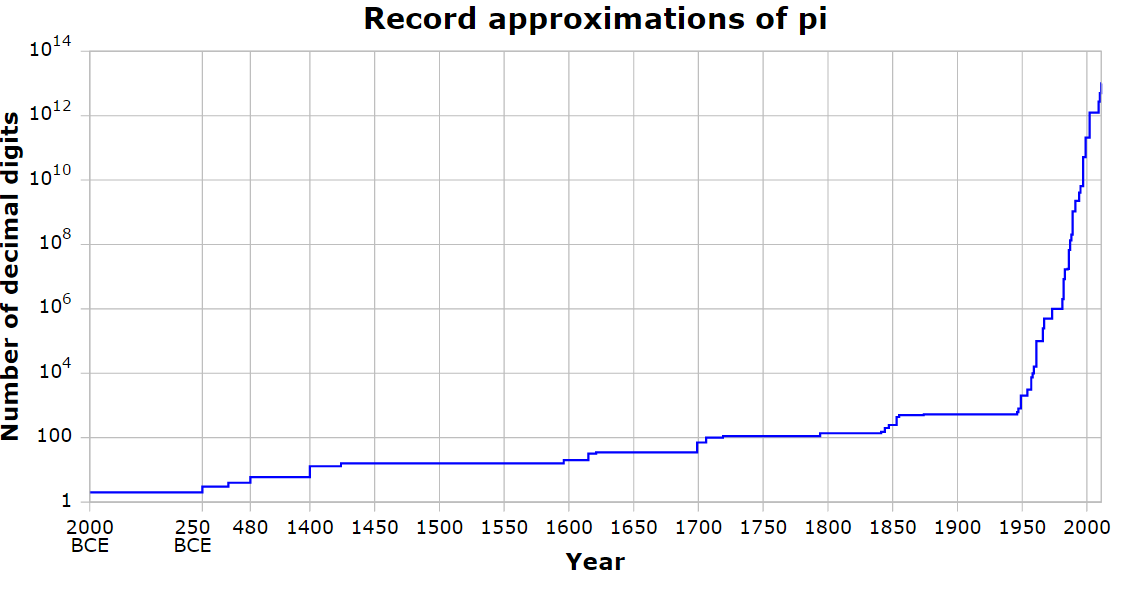
\includegraphics[width=3.5in, height=2.5in]{pidigits.png} 
\end{center}

\begin{questions}

%%%%%%%%%%%%%%%%%%%%%%%%%%%%%%%%%%%%%%%%%%%%%%%%%%%%%%%%%%%%%%%%%%%%%
\question Taylor series are a major tool used to calculate digits of $\pi$, specifically, the following series for arctangent.
\[
\arctan(x) = \sum_{n=0}^{\infty} (-1)^n\frac{x^{2n+1}}{2n+1}, \quad\quad R=1, \quad\quad IoC = [-1,1]
\]
Derive this series for arctangent by using a geometric series. Explain why the radius of convergence is $R=1$. Explain why the interval of convergence is $[-1,1]$. \\ \ \\
Hint: For the interval of convergence, you need to check the endpoints separately using a series test from Calculus II.

\pagebreak


%%%%%%%%%%%%%%%%%%%%%%%%%%%%%%%%%%%%%%%%%%%%%%%%%%%%%%%%%%%%%%%%%%%%%
\question Using the arctangent Taylor series from the previous problem, one can create a series approximation for $\pi$ from the following three formulas.
\begin{align}
\frac{\pi}{4} &= \arctan(1) &\text{(leads to Leibniz's formula for $\pi$)}\\
\frac{\pi}{4} &= \arctan\left(\frac{1}{2}\right) + \arctan\left(\frac{1}{3}\right) &\text{(leads to Euler's formula for $\pi$)}\\
\frac{\pi}{4} &= 4\arctan\left(\frac{1}{5}\right) - \arctan\left(\frac{1}{239}\right) &\text{(leads to Machin's formula for $\pi$)}
\end{align}
There are countless others which can be created in this way. 
\begin{parts}
\part Verify the identity (1).
\part Using the Taylor series for arctangent, program each of the three formulas in Scilab. Compare and contrast the performance of each. How fast are they? How many terms of the series are needed for exact digits of $\pi$? Find the absolute error at each step. The first is rather slow. What do you think the reason is?
\end{parts}


%%%%%%%%%%%%%%%%%%%%%%%%%%%%%%%%%%%%%%%%%%%%%%%%%%%%%%%%%%%%%%%%%%%%%
\question With problem 2, you are limited to machine precision (about 16 decimal digits in Scilab). So how do you get more digits of $\pi$? I have attached a script written in Matlab which accomplished this task.
\begin{parts}
\part Translate this script into Scilab and run it.
\part Give a complete explanation as to how the script works. You should understand every line of code and the role it plays. This script uses the same strategy as was used with the very first $\pi$ computation via a computer as accomplished by Jon von Neumann in 1949. See the paper on D2L for the story of this 1949 computation.
\part Compare each of the three formulas from problem 2 using your new many digit program. 
\end{parts}

%%%%%%%%%%%%%%%%%%%%%%%%%%%%%%%%%%%%%%%%%%%%%%%%%%%%%%%%%%%%%%%%%%%%%
\question OPTIONAL challenge problem. Derive the last two formulas given in problem 2 using some trigonometric fantasticness.

\end{questions}
\end{document} 